%/*******************************************************************************
% * Copyright (c) 2007, G. Weirich
% * All rights reserved. This program may not be distributed
% * or modified without prior written consent
% *
% * Contributors:
% *    G. Weirich - initial implementation
% *
% *  $Id: anleitung.tex 231 2007-08-23 19:12:43Z Gerry $
% *******************************************************************************/

\documentclass[a4paper]{scrartcl}
\usepackage{german}
\usepackage[utf8]{inputenc}
\usepackage{makeidx}
\usepackage[pdftex]{graphicx}
\DeclareGraphicsExtensions{.pdf,.jpg,.png}
\makeindex
\usepackage{floatflt}
\usepackage[]{hyperref}
\usepackage{color}
\title{Stammdatenimport von Aeskulap nach Elexis\textsuperscript{\textregistered}}
\author{Gerry Weirich}

\begin{document}
\maketitle
\section{Einführung}

Dieses Plugin ermöglicht Ihnen den Import von Stammdaten aus dem Arztpraxisprogramm 'Aeskulap'.
Zur Installation kopieren Sie das Plugin einfach in Ihr Plugins-Verzeichnis.

\section{Voraussetzungen}
Dieses Plugin benötigt Elexis 1.4.0 oder höher.

\medskip

Die in Aeskulap enthaltenen Stammdaten können nur von Aeskulap selbst exportiert werden, da das Datenformat nicht öffentlich ist. Es gibt bisher unseres Wissens zwei Möglichkeiten:
\begin{itemize}
  \item Über das Menu von Aeskulap selbst: \textsc{Stammdaten- Krankengeschichte - KG-Filter}, dann Suchkriterien eingeben und exportieren. Sie erhalten ein CSV-File, das allerdings nur die Personalien enthält. Sie können den Export so konfigurieren, dass nur Männer oder nur Frauen, oder alle Patienten exportiert werden. In letzterem Fall muss Elexis das Geschlecht der so importierten Patienten 'erraten'.
  \item Sie bitten Ihren Aeskulap-Supporter, die Stammdaten für Sie als Excel 97-Dateien zu extrahieren. Sie erhalten fünf Dateien mit den Namen 'adressen.xls', 'firma.xls', 'garant.xls', 'pat.\_garanten.xls' und 'patienten.xls'. Dies ergibt eine umfangreichere Datenbasis, die beispielsweise auch Kostenträger erfasst. Dies ist deshalb im Zweifelsfall vorzuziehen.
\end{itemize}

\section{Verwendung}

\begin{figure}
    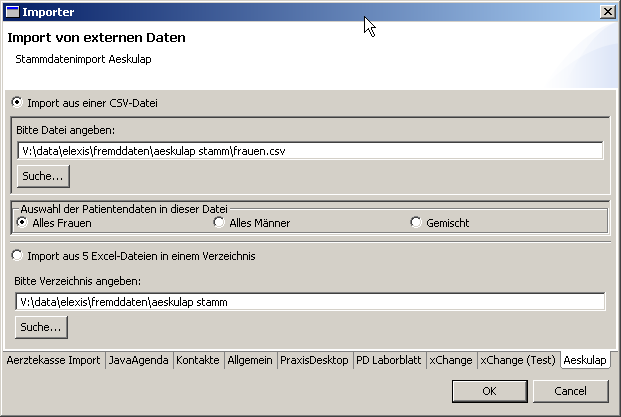
\includegraphics[width=0.8\textwidth]{aeskulap}
    \caption{Aeskulap-Import}
    \label{fig:aeskulap}
\end{figure}


Wenn der Aeskulap-Importer korrekt installiert ist, erscheint er automatisch im Menu \textsc{Datei-Datenimport}. Wählen Sie dort den Reiter 'Aeskulap' aus (Abb. \ref{fig:aeskulap}). Klicken Sie je nach Importquelle (s. unter 'Voraussetzungen') auf den Auswahlknopf \textsc{Import aus CSV-Datei} oder \textsc{Import aus 5 Excel-Dateien}. Klicken Sie dann auf den dazugehörigen 'Suche...' Knopf und wählen sie die gewünschte Importdatei resp. das Verzeichnis, in dem die 5 benötigten Dateien sind aus.
Falls Sie aus einer CSV-Datei importieren, sollten Sie ausserdem noch angeben, ob die Datei nur Frauen, nur Männer oder beides enthält.

Klicken Sie dann auf ok. Je nach Umfang der Daten wird der Import einige Sekunden bis Minuten dauern.

\bigskip

Nach dem Import können Sie das Import-Plugin wieder löschen, es wird nicht mehr benötigt.

\section{Zusammenlegen mehrerer Datenbanken}
Sie können dieses Plugin selbstverständlich auch verwenden, um mehrere Datenbanken, beispielsweise bei der Zusammenlegung von Praxen, zusammenführen. Es wird beim Import keine Kollisionen und keine Datenverluste geben, aber es kann dann vorkommen, dass einige Patienten mehrfach in die Datenbank gelangen. Eine Erweiterung des Plugins, die identische Patientendaten erkennen kann, wäre natürlich bei Bedarf möglich.

\end{document} 